%ब
\chapter{Implementation} \label{c:Implementation}


\section{Experimental API}\label{s:API}

The experimental \ac{API} is designed generically in order to ensure
that it can be used by  applications to maintain dependencies within their
keyspaces irrespective of keyspace schemas or structures of column
families. However, applications using this \ac{API}  have to provide
 the metadata information relevant to the constraints of their keyspace as
 explained in the previous section. 
% Thus,  this \ac{API} is made adaptable to different keyspace schemas  that can
% be deployed in column-oriented key-value \acp{DBMS}.  

This \ac{API} validates the referential integrity based on the metadata provided
for the application and its column families.  It  provides  four solutions
with different approaches to meet different requirements. However, with 
 every one of these solutions,  the referential integrity constraint is
 implemented in Cassandra.

The  class diagram of the \ac{API} is presented seen in
 Figure~\ref{f:classDiagram} alongside with the example classes that belong to 
the University keyspace. The main components are the Entities, Entity Managers,
and Validation handlers, all of which are described in the next sections.  
 Notice that for the sake of clarity and brevity,  the class diagram only
 contains  the relevant  methods of the classes, favoring a simpler
explanation of the functioning of the \ac{API}.

\begin{figure}[h]   
	\centering
	%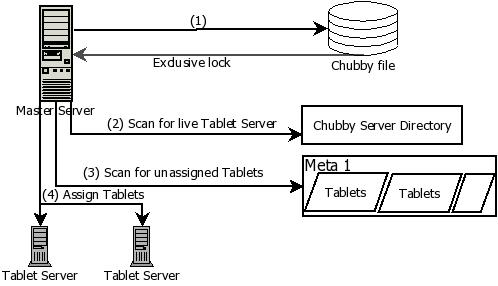
\includegraphics[width=5cm,   height=5cm]{. /figure/random. jpg}
	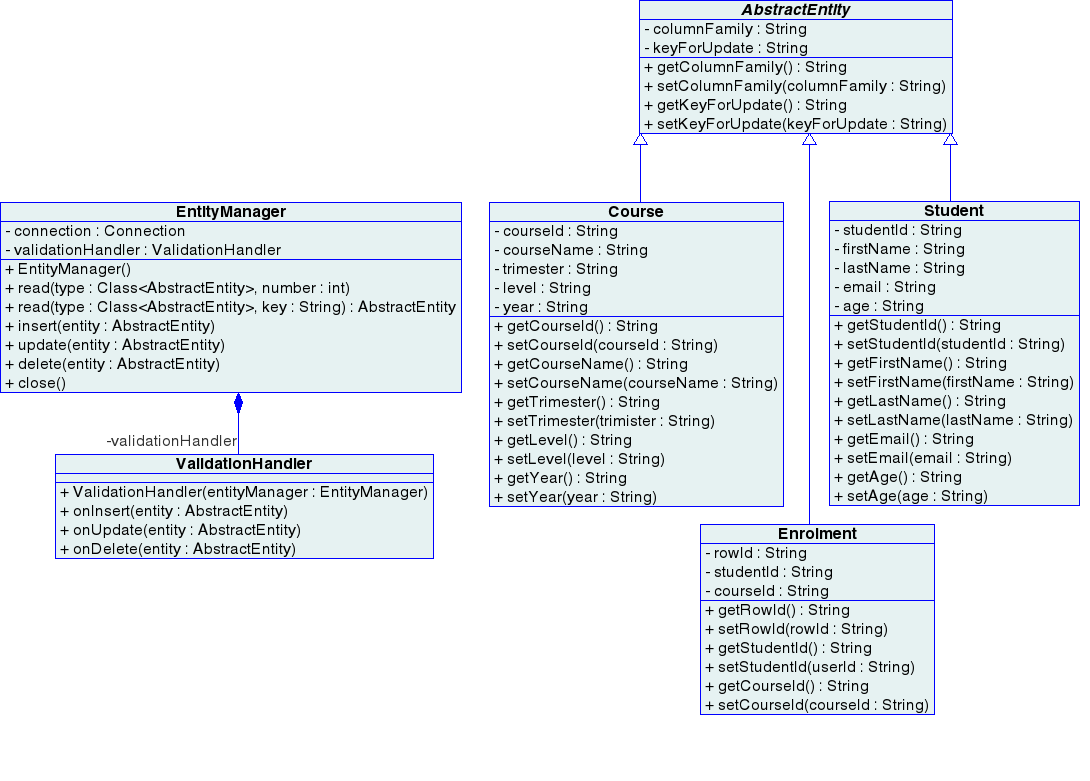
\includegraphics[width=\textwidth]{./figure/Solutions/FinalClassDiagram.png}
	\caption{Class Diagram for the \ac{API}}\label{f:classDiagram}
\end{figure}


	\subsection{Entities} 
	
	An entity class contains attributes (with respective getters and setters) that
	map columns within a specific column family. As such, the contents of a
	column family can be represented by a list of entity objects. All entities in
	the \ac{API} extend from the abstract class \texttt{AbstractEntity} which
	contains attributes (and respective getters and setters) to
	aid the \ac{API} towards their management. Particularly, the attributes
	that \texttt{AbstractEntity} contains  are \texttt{columnFamily} which
	determines the column family to which the entity maps, and 
	\texttt{keyForUpdate} which shall contain the new value in case the primary key
	of the entity is to be updated.
	
	For example,  considering the University keyspace example, \texttt{Enrolment} 
	is an entity class that  maps the \texttt{Enrolment}  column family and
	it contains the attributes \texttt{RowId}, \texttt{CourseId} and
	\texttt{StudentId} which represent the respective columns. As such, an instance
	of \texttt{Enrolment} contains the values of one super column. Likewise,
	\texttt{Student} and \texttt{Course} are entity classes and their instances 
	map to the respective super columns in their column families.
% 	For all the solutions in this \ac{API},  entities of the user applications are
% 	designed to extend the abstract class called \texttt{AbstractEntity},  which has
% 	information about the  methods for accessing and defining  entities.  For
% 	every column family, applications derive a class from the
% 	\texttt{AbstractEntity} containing attributes.
	The \ac{CRUD} operations that can be performed on these entities   are
	handled by the \texttt{EntityManager},  which is described next.
		
	\subsection{EntityManager}

	The  \texttt{EntityManager} class implements  all
	the \ac{CRUD} operations to be performed on the entities. In order to perform
	these operations,  the \texttt{EntityManager} interacts with the respective
	keyspace the entity belongs. Moreover, it ensures to trigger the   referential
	integrity validation process whenever a \ac{CRUD} operation requires it. This
	is performed by creating a  \texttt{ValidationHandler} (explained in the next
	section) and passing the entity to be checked for constraint violations. 
	
	The \texttt{EntityManager}, before performing any operation, requires a
	connection to the keyspace. This connection is established using a third-party
	\ac{API} named Hector (freely available at \todo{www.hector.com}). Hector
	 encapsulates the driver-level interface provided by Cassandra (named Thrift) 
	 and simplifies the interaction with it. Regarding the \ac{CRUD} 
	 operations, Hector provides  a \texttt{Mutator} object which encapsulates the
	 necessary procedures to interact with the Cassandra cluster.    
	 
	 Notice that  the \texttt{EntityManager} is able to generically deal with any
	 entity that derives from \texttt{AbstractEntity}. It does so by using
	 reflection (a Java  feature) to detect the attributes of an object and
	 generically invoking the getters and setters of the entities. Thus, the
	 \texttt{EntityManager} is able to perform all \ac{CRUD} operations on
	 any entity. These operations are explained in detail next.  
	 
	 
	
% 	Hector is a high
% 	 level client that wraps the driver-level interface of Cassandra called Thrift.
% 	 Hector  provides some features that  Thrift does not, for example, 
% 	 fail-over mechanisms and connection pooling (\todo{cite book}).  
	 % 	 While there
% 	 are other wrappers for Thrift, Hector was  chosen as  it is one of the
% 	 earliest wrappers and  encapsulates the interaction with the Thrift \ac{API}
% 	 and makes it simpler to access a Cassandra cluster.	
	
	
	
	
		\subsubsection{Create}
		 The \texttt{create} (or \texttt{insert}) operation stores entities in the
		 respective column families. The \texttt{EntityManager} inserts these entities
		into the column families represented by the entity class.  
		For example,  all the student entities are inserted into the column family
		\texttt{Student} through the \texttt{EntityManager}. 
		
		The \texttt{EntityManager} passes the entity details which include entity key
		and column family information as parameters to the \texttt{addInsertion}
		method of the \texttt{Mutator}.  The \texttt{insert} operation triggers a
		 referential integrity validation whenever a child entity is  inserted in
		 order to ensure that its parent entities exist. The validation is performed
		 by the \texttt{onInsert} method of \texttt{ValidationHandler}, which is
		explained in Section~\ref{ss:VH}.
	
		\subsubsection{Read}
		The  \texttt{read} operation retrieves  entities from a keyspace given the
		entity class. This operation does not prompt any referential integrity validation since
 		entities are only read and their state is not changed, unlike in the other
		operations.
		
% 		\todo{talk about mutator CONSISTENCY}
		
		This \ac{API} provides two methods for retrieving entities. One retrieves a
		single entity given its class and the value of the respective primary key. The
		other retrieves a list of entities representing the contents of
		the column family.

		
		
		\subsubsection{Update}\label{ss:update}
		In an \texttt{update} operation the existing contents of an entity are merged
		with new contents.  In other words, the  values of their columns they
		represent are updated to new values and committed into the column families.  
		 The \texttt{EntityManager} provides two types of updates, one in which it
		 uses the primary key of the entity to update it, and the other one in
		 which uses the especial field \texttt{keyForUpdate} to update the primary as
		 well as the rest of the fields. 
		 
		 If the entity to be updated does not contain a change in its primary key, a
		 normal update takes place. Otherwise, referential integrity needs to be
		 ensured. In order to do so, the following steps are performed:
% 		 In order to do so, the \texttt{EntityManager} passes the entity
% 		 to the \texttt{ValidationHandler}  to check for referential integrity, 
% 		 retrieves the list of child entities that depend on its primary key, deletes
% 		 dependencies and the entity,  and update the dependencies Following this, the
% 		 steps that are performed are :
		\begin{enumerate}
		  \item Check with the \texttt{ValidationHandler} if the entity can be
		  updated.
		  \item Retrieve the list of child entities that depend on the previous
		  primary key of the entity to be updated.
		  \item Perform \texttt{delete} on the child entities from their column family
		  in Cassandra.
		  \item Perform a \texttt{delete} on the entity with the primary key from the
		  column family.
		  \item Perform an \texttt{insert} with the entity and its new primary key.
		  \item Update the foreign keys in the child dependencies to
		  the new value.
		  \item Perform an \texttt{insert} operation to reinsert the child entities
		  into their respective column families.
		\end{enumerate}
		
% 		In all the solutions,  an \texttt{Update} operation triggers a referential
% 		 integrity validation whenever any primary or foreign keys of any entities are
% 		updated.
% 		The validations are performed by the \texttt{onUpdate} method of the
% 		\texttt{ValidationHandler}.
		
		Notice that such procedure is used as a workaround of the restriction of
		Cassandra to change a primary key. Once a record has been
		inserted into the column family, the primary key cannot  be changed. This is
		known as a tombstone delete, which prevents aside from changing a primary
		key, deleting a primary key.
		
		\subsubsection{Delete}\label{ss:delete}
		In a  \texttt{Delete} operation, entities are removed from a column
		family. As mentioned before, due to the tombstone delete, the primary key
		will never cease to exist, but the values of the columns are emptied. 
		
		In all the solutions,  a \texttt{Delete} operation triggers a referential
		integrity validation every time a parent entity is deleted.  This validation
		is performed by the \texttt{onDelete} method of the
		\texttt{ValidationHandler}, which is explained in next section. 
		 
		 The 	\texttt{EntityManager} passes the entity information to the
		\texttt{delete} method of the \texttt{Mutator} object.
 		
%  		Before a parent entity is deleted, the \texttt{EntityManager} retrieves the
%  		child entities it depends upon  from he \texttt{ValidationHandler} if the
%  		 referential intergity is not violated. The \texttt{EntityManager} deletes
%  		the child entities prior to deleting the parent entity.
		
		\subsection{ValidationHandler}\label{ss:VH}
		The \texttt{ValidationHandler} is invoked by the \texttt{EntityManager} every time
		an operation triggers a
		referential integrity validation on any entity. 
		The \texttt{EntityManager} passes the entity and the connection details  to
		the \texttt{ValidationHandler} to perform the validation.
		
		The \texttt{ValidationHandler} contains the  logic for checking whether an
		 entity has any dependencies and verifies whether an \texttt{insert},
		 \texttt{update} or \texttt{delete} operation  violates the referential
		integrity or not.  To ensure that these operations maintain referential
		 integrity between entities, it applies the appropriate referential integrity
		 rules, as explained in Section~\ref{s:referential-integrity}. Thus, for an
		 \texttt{insert} operation the insert rule of referential integrity is
		 followed and similarly for \texttt{update} and \texttt{delete} operations
		 their respective rules are applied. As previously mentioned, a \texttt{read}
		 operation does not invoke any referential integrity validation in this
		 \ac{API}. The referential integrity validation performed by
		 \texttt{ValidationHandler} for each of these operations is discussed next
		with pseudocodes.
		
		\begin{description}
		\item[onInsert]: 
		In an \texttt{insert} operation a referential
		integrity validation is triggered whenever a child entity is  inserted. 
		The \texttt{ValidationHandler} applies the referential integrity insert
		rule which checks whether  valid parent entities with
		primary keys matching the foreign keys of the child entities exist, else an
		exception is raised stating that the referential integrity has been violated.
		Thus, the following checks are performed by the \texttt{ValidationHandler}.
		\renewcommand{\labelenumii}{\arabic{enumi}.\arabic{enumii}}
		\renewcommand{\labelenumiii}{\arabic{enumi}.\arabic{enumii}.\arabic{enumiii}}
		
		\begin{enumerate}
		\item if entity has \ac{FK} constraints
				\begin{enumerate}
				\item Identify parent entity class from the \ac{FK} constraint.
				\item if foreign keys exist as  primary key in  parent entity class
				  		\begin{enumerate}
				  		\item \texttt{EntityManager} inserts the entity.
				  		\end{enumerate}
				\item else
				   		\begin{enumerate}
				   		  \item Raise exception and cancel \texttt{insert}.
				   		\end{enumerate}
				\end{enumerate}   	
		\item else if no \ac{FK} constraints exist
		  		\begin{enumerate}
		  		\item \texttt{EnityManager} inserts entity.
		  		\end{enumerate}
		\end{enumerate}
		The implementation of the \texttt{insert} operation is consistent across all the
		solutions. 
		\item[onUpdate:] The validation for an \texttt{update} operation is different
		when primary keys and foreign keys are updated. 
		\begin{description}
		\item[Case A: Update Primary Key] When a  primary key of a
		parent entity is updated, the \texttt{ValidationHandler} performs the
		following checks.
		\renewcommand{\labelenumii}{\arabic{enumi}.\arabic{enumii}}
		\renewcommand{\labelenumiii}{\arabic{enumi}.\arabic{enumii}.\arabic{enumiii}}
		%\renewcommand{\labelenumiiii}{\arabic{enumi}.\arabic{enumii}.\arabic{enumiii}.\arabic{enumiiii}}
		\begin{enumerate}
		  \item if \ac{FK} constraints on primary key exist
		  	\begin{enumerate}		  	
		    \item if \texttt{DeleteRule} for the \ac{FK} constraint is
		    \texttt{Cascade}
		    	\begin{enumerate}
		    	  \item Pass any existing child entities to the \texttt{EntityManager} to
		    	  allow update of both primary and foreign keys.
				\end{enumerate}
			\item else if \texttt{DeleteRule}  is \texttt{NoDelete}
				\begin{enumerate}
				  \item if no child entities exist
				  		\begin{enumerate}
				  		  \item \texttt{EntityManager} performs update on  the primary key.
				  		\end{enumerate}
				  \item else if child entities exist
				   		\begin{enumerate}
				    	\item Raise exception and rollback \texttt{update}. 
				    	\end{enumerate}
				\end{enumerate}
			\end{enumerate}
		  \item else if no \ac{FK} constraints are found 
		  		\begin{enumerate}
		  		  \item \texttt{EntityManager} performs update on the primary key.
				\end{enumerate}
		 \end{enumerate}
		 
		For example,  in the University keyspace,  when a
		new \texttt{StudentId} is provided for an existing  \texttt{Student}
		entity,  then \texttt{ValidationHandler}
		checks metadata and locates the \ac{FK} constraint \texttt{CONST400} as seen in
		Figure~\ref{f:metadataInSolutions}. Since the \texttt{DeleteRule} is
		\texttt{Cascade}, the \texttt{EntityManager} allows the \texttt{update}
		operation to take place as explained in the EntityManager section.
			
% 			For example, when the foreign key \texttt{StudentId} for one of the entities
% 		in \texttt{Enrolment} is given a new value,  then the \texttt{ValidationHandler} 
% 		identifies the parent entity class for its \ac{FK} constraint
% 		\texttt{CONST400} as \texttt{Student}.  If the new \texttt{StudentId} 
% 		exists as a primary key for any
% 		 of the  entities in \texttt{Student} entity class,  the \texttt{update} is
% 		 performed.
		 
		\item[Case B: Update Foreign Key] When a foreign key of a child entity is
		updated, the  \texttt{EntityManager} performs the same check on the
		metadata and locates its \ac{FK} constraints. It then follows these steps:
		\begin{enumerate}
		  \item Identify parent entity class from the \ac{FK} constraint.
		  \item if new foreign keys exist as primary key in parent entity class
			\begin{enumerate}
				\item \texttt{EntityManager} updates  the foreign key.
			\end{enumerate}
		  \item else 
			\begin{enumerate}
				\item Raise exception.
			\end{enumerate}
		\end{enumerate}

	
		
		\end{description}
		The implementation of the \texttt{update} operation for both the cases is
		consistent for all solutions.
		
		\item[onDelete:] In a \texttt{delete} operation a referential
		integrity validation is triggered whenever an entity is deleted. The
		\texttt{ValidationHandler} applies the referential integrity delete rule
		and performs the following checks:
		\renewcommand{\labelenumii}{\arabic{enumi}.\arabic{enumii}}
		\renewcommand{\labelenumiii}{\arabic{enumi}.\arabic{enumii}.\arabic{enumiii}}
		
		\begin{enumerate}
		  \item Identify existing \ac{FK} constraints on the entity.
		  \item if \ac{FK} constraints exist,
		  		\begin{enumerate}
		  		  \item if \texttt{DeleteRule} is \texttt{Cascade}
		  		 		\begin{enumerate}
		  		 		   \item Pass any existing child entities to the \texttt{EntityManager}
		  		 		   to allow delete of child  and parent entities.
		  		 		\end{enumerate}
		  		  \item else if \texttt{DeleteRule}  is \texttt{NoDelete}
						\begin{enumerate}
						  \item if no child entities exist
						  		\begin{enumerate}
						  		  \item \texttt{EntityManager} deletes the entity.
						  		\end{enumerate}
						  \item else if child entities exist
						   		\begin{enumerate}
						    		\item Raise exception. 
						    	\end{enumerate}
						\end{enumerate}
						
				  \item else if no \ac{FK} constraints are found 
				  		\begin{enumerate}
				  		  \item \texttt{EntityManager} deletes the entity.
						\end{enumerate}
		  		\end{enumerate}
		\end{enumerate}	
		For example,  in the University keyspace,  if a 
		\texttt{Student} entity in \texttt{Student} column family is marked for
		deletion, the \texttt{EntityManager} locates the \ac{FK} constraint 
		\texttt{CONST400} referencing \texttt{Student}.
		Since the \texttt{DeleteRule} is \texttt{Cascade}, 
		the child entities are deleted from \texttt{Enrolment} prior to deleting the
		entity from its \texttt{Student} column family. 
		\end{description}
		
% 		
% 		Since metadata is stored differently in the solutions, the operation for
% 		retrieving the metadata in the  \texttt{ValidationHandler} is different for
% 		each solution in the \ac{API}. 
% 		 For example,  the \texttt{ValidationHandler}
% 		for Solution 1 and 2 involves parsing the metadata  since it is stored as a
% 		 \texttt{String} along with the actual data while in Solution 3 and 4 it is
% 		 saved as an entity class.
% 		
		The referential integrity validation logic, implementation of the \ac{CRUD}
		operations and Cassandra connection settings are common for all the solutions
		in the \ac{API}.
		
		The following sections describe each of the four solutions in terms of how
		these store ,decipher, access and retrieve the metadata. The motivation for
		each of the solution is also discussed. 
% 		how metadata is accessed and retrieved
% 		and the motivation for the solution's design.


	
\section{Solution 1:  Metadata with Special Characters}\label{s:sol1-real}

\subsection{Metadata Storage}
	This solution saves the metadata embedded with the actual data and is stored in
	the column family belonging to the actual data. This means that metadata is
	included in every super column in a column family as the value of column
	\texttt{Metadata}. Since metadata is common for all the entities in an entity
	class, every super column contains the same metadata value for this column.For
	example, in the University keyspace, metadata in \texttt{Student} is stored in
	every super column as seen in Figure~\ref{f:sol1-Student-md}.
	
		\begin{figure}[H]
			\centering
			%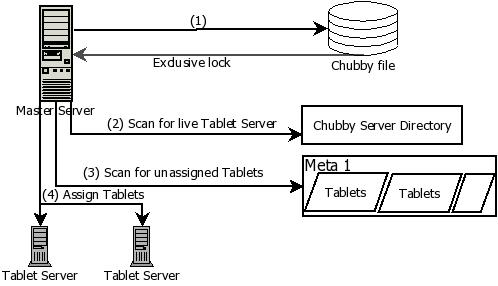
\includegraphics[width=5cm,   height=5cm]{. /figure/random. jpg}
			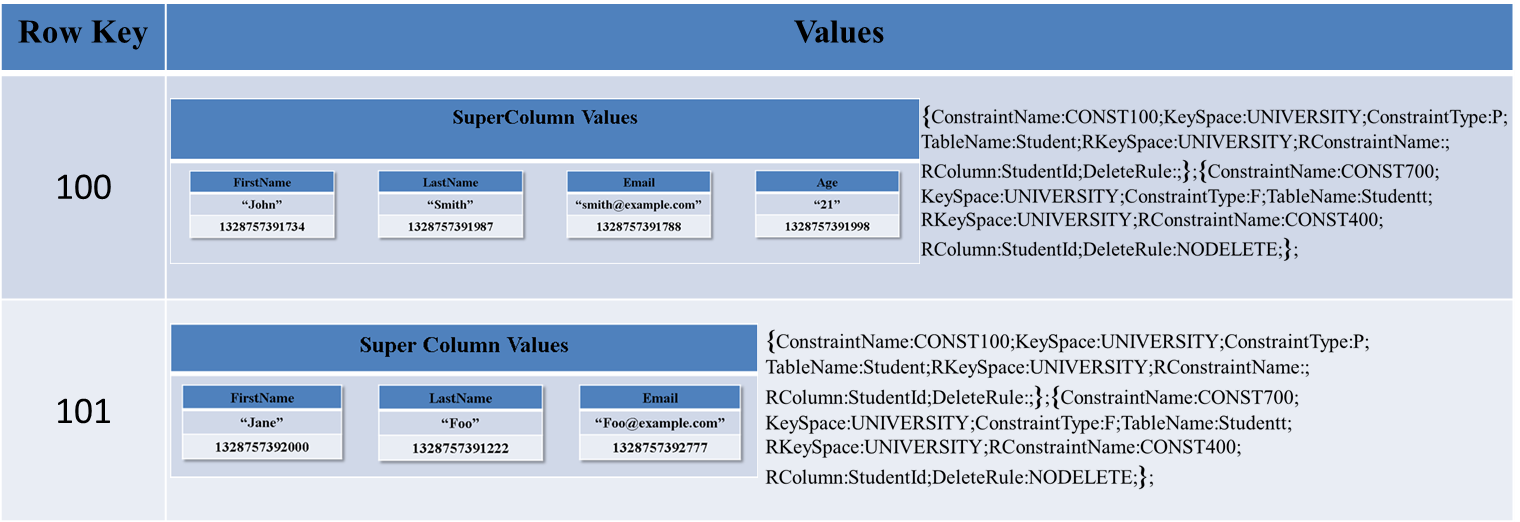
\includegraphics[width=1\textwidth]{./figure/Solutions/Solution1-Student-MD.png}
			\caption{Metadata storage in Solution 1}\label{f:sol1-Student-md}
		\end{figure}
		
	In this solution, the structure of the constraints in metadata is as described
	in Section~\ref{s:Metadata} and each entity class stores  its \ac{PK}
	constraint and related \ac{FK} constraints in the metadata. 
	Each entity stores the following constraints as its metadata.
	
		\begin{itemize}
		  \item  \ac{PK} constraint showing the primary key of the column family.
		  \item \ac{FK} constraints 
				\begin{itemize}
					\item In the case of a parent entity the \ac{FK} constraints are the \ac{FK}
					constraints of type '\texttt{F}' to identify the child entities when the entity
					is being updated or deleted.
					\item  In the case of a child entity the \ac{FK} constraint of type '\texttt{R}'
					is stored to indicate the parent entities.
					\item If an entity is both a parent and a child, then its metadata
					stores its \ac{PK} constraint and the \ac{FK} constraints of both types.
				\end{itemize}
		\end{itemize}
		
	For instance, \texttt{Student}  is a parent entity with a child dependendent on
	it, namely \texttt{Enrolment}. 
	Its metadata thus contains its \ac{PK} constraint \texttt{CONST100} and the
	\ac{FK} constraint \texttt{CONST700}. Since
	\texttt{Enrolment} is a child entity it  stores its \ac{PK} constraint
	\texttt{CONST300} and its \ac{FK} constraints \texttt{CONST400} and
	\texttt{CONST500}. Similarly, other entities like \texttt{Course} store its
	\ac{PK} and respective \ac{FK} constraints.
	
	Special characters are used within the metadata to separate the constraints and
	to identify its different parts. The special characters used in this solution
	are '\texttt{\{}', '\texttt{\}}','\texttt{;}' and '\texttt{:}'. The special
	characters are used the following way:
	
	\begin{itemize}
	\item Each constraint is enclosed in curly brackets and separated from each
	other by the special character '\texttt{;}'. For example,in \texttt{Student}
	\texttt{CONST100} and \texttt{CONST700} are enclosed in curly braces and
	separated by '\texttt{;}'. Thus, '\texttt{\};}' marks the end of every
	constraint in the metadata.


	\item The different parts of each constraint are separated by the special character
	'\texttt{;}'. For example,  '\texttt{;}' separates the \texttt{ConstraintName}
	 and \texttt{Keyspace} and other parts in the constraints \texttt{CONST100} and
	 \texttt{CONST700}
	 
	 
	\item Each part and its value are separated by the special character
	'\texttt{:}'. For example, \texttt{ConstraintName} is separated from
	its value \texttt{CONST100} with a \texttt{:}. This helps in identifying the
	name and value for every part while parsing the metadata information
	in the \ac{API}.
	
	\end{itemize}
	
\subsection{Metadata Retrieval}
	In this solution, the metadata is read as a String by the
	\texttt{AbstractEntity} and it is parsed to extract the diffrent parts and its
	values. All the special characters used within the metadata become the
	delimiters for the String parsing and  the different parts and
	its values are converted to tokens. 
	The delimiters used for parsing are:
		\begin{itemize}
		  \item Special characters '\texttt{\{}', '\texttt{\}}' and '\texttt{;}' are
		  the delimiters for extracting each constraint from the metedata.
		  \item Special character '\texttt{;}' is the delimiter for identifying each
		  part within a constraint.
		  \item Special character '\texttt{:}' is the delimiter for extracting the
		  field name and the value from each part of the constraint.
		\end{itemize}
		
	In this solution, an enity class for metadata with the required getter and
	setter access methods is created and used to save the metadata of an entity
	whenevr any operation is invoked on it.
	The \texttt{AbstractEntity} treats metadata just like an entity and sets the
	tokenised values using the metadata entity's setter methods.
	Every time an operation is invoked on an entity the \texttt{EntityManager}
	retreves the metadata from the \texttt{Metadata} column of the entity and loads
	it as text.
		 
	 
	 
\subsection{Metadata Access}
	  
 For referential integrity validation the
	 \texttt{ValidationHandler} accesses each part of the metadata using the
	 relevant setter methods. For instance, to get information of
	the \texttt{DeleteRule} of a constraint on the entity,
	\texttt{ValidationHandler} uses the \texttt{getDeleteRule} method of the
	metadtaa entity class and likewise for all the other different parts
	of the metadata respective getter methods are used.
	 
	 The logic for the referential
	 integrity validation by the \texttt{ValidationHandler} once the String metedata is parsed is the same as described in Section~\ref{ss:VH}.

	In this solution, the metadata is saved  when entities are inserted into the
	column family and thus the metadata is a part of each of the entity.  Since the
	metadata is present as the value in every super column,  accessing the metadata
	information for referential integrity validation is as simple as accessing the
	value itself,  requiring no additional actions or connection to the
	keyspace. Saving the metadata as embedded metadata in this solution is useful
	as entities are replicated across the distributed cluster, making metadata
	easily accessible by every node in the cluster, since it is a part of the
	entity.

	The \ac{API} parses the metadata of an entity by reading any of its
	instances and need not load metadata from any external location.

	On the other hand,  the metadata for an entity would be the same for all its
	instances .  For example,  in the University example,  the metadata
	information for the \texttt{Student} entity is applicable to each of its
	instances,  indicating that each instance  should have a primary key called
	\texttt{StudentID}.
	Similarly,  all \texttt{Course} instances have the same \ac{PK} constraints
	applied on it.  When metadata is saved as a part of the  value,
	every instance of an entity will contain the constraint information
	in it's value.  Since the metadata information and constraints are same for all
	the instances of a single entity ,  this metadata is repeated every time an
	instance of the entity is inserted.  For example,  if
	\texttt{1000} \texttt{Student} instances are inserted,  the metadata for these
	\texttt{1000} instances are saved \texttt{1000} times too, along with these
	instances.  But the metadata is exactly same for all the
	instances \todo{(Figure~\ref{})}.


	The distributed nature of cloud \ac{NoSQL} \acp{DBMS} also means that the
	metadata is not only repeated several times within the same column family,  but
	also across the nodes in the cluster, thus increasing the redundancy of
	the metadata.  But such a redundancy and consumption
	of space to store the metadata is not a potential issue
	in cloud column-oriented key-value \acp{DBMS}, since storage on the cloud is
	inexpensive and  does not affect the economic benefits.

	Such a storage mechanism is not expected to affect the efficiency of the
	cluster negatively as the metadata information is not large in size and is
	easily replicated along with the actual data and does not exert any extra
	resources in the cluster.  The performance of this solution is analysed  in
	Chapter~\ref{}.

	Much research has been done in the area of  metadata management in distributed
	environments,  where emphasis is laid on the synchronous updates of metadata
	storage as well as its efficient storage and access mechanisms(\todo{cite more}
	Hackl et al.  2010).
	In Hackl et al.  (2010),  metadata management is discussed in the context of
	huge file systems, where metadata is stored separately in a suitable \ac{DBMS}
	so that such file systems can be managed and administered efficiently without
	slowing them down.  To analyse which type of \ac{DBMS} was more suitable for such a
	metadata storage,  they conducted various experiments and concluded that
	key-value \acp{DBMS} were more efficient in terms of speed,  memory and resource
	consumption when compared to popular \acp{RDBMS}.  As a part of their
	experiments, they adopted an interesting approach to store metadata in a
	key-value \ac{DBMS} ,  namely Tokyo Cabinet,  a popular \ac{NoSQL} \ac{DBMS}
	that stores records as simple key-value pairs in data files. Unlike Cassandra,
	tokyoCabinet does not involve data types or columns
	and so on (\todo{cite}).  In their approach,  metadata about the file system
	used in their experiment is inserted as a value which is associated with a unique key and the
	different parts of the metadata are separated by semicolons (Hackl et al.  2010).
	

\section{Solution 2:  Metadata as Top Row}\label{s:sol2-real}
	
	\subsection{Metadata Storage}
	This solution saves the metadata embedded with the actual data and exists in
	the same column family as the data. This approach is similar to
	Solution~1 where metadata is stored within the same column family. But unlike
	Solution~1, this solution saves the metadata only once in the column family as a
	top row or the first super column in a column family with the unique
	\texttt{RowId} '\texttt{-1}'. This top row has only a single column 
	\texttt{Metadata}  containign the metadta information and this is  unlike
	other super columns which have different columns. This is possible since
	Cassandra allows rows to have different number of columns, as described in
	Section~\ref{s::key-value-data-model}. Thus, for each entity class, the
	metadata exists only once as a single row and is common for all the instances
	of the entity.
	In the University example  a \texttt{Student} entity has the
	metadata  stored as a top row in Figure~\ref{}.
		 
	\begin{figure}
	\todo{ Insert metadata top row figure for Student}
	\end{figure}
		
	The metadata in this solution contains
	special characters '\texttt{\{}', '\texttt{\}}','\texttt{;}' and '\texttt{:}'
	to distinguish all the constraints and its different parts and values.
	The metadata stored for each column family has the following
	constraints:
	\begin{itemize}
	  \item  \ac{PK} constraint showing the primary key of the column family.
	  \item \ac{FK} constraints 
			\begin{itemize}
				\item In the case of a parent entity the \ac{FK} constraints are the \ac{FK}
				constraints of type '\texttt{F}' to identify the child entities when the entity
				is being updated or deleted.
				\item  In the case of a child entity the \ac{FK} constraint of type '\texttt{R}'
				would be stored along with the \ac{PK} constraint which indicates its parent
				entities.
				\item If an entity is both a parent and child entity, then its metadata would
				hold its \ac{PK} constraint, and the \ac{FK} constraints of both types.
			\end{itemize}
	\end{itemize}
	
	Consider \texttt{Enrolment}  which is a child entity with parent entities
	\texttt{Student} and \texttt{Course} (Figure~\ref{}). Its metadata thus
	contains its \ac{PK} constraint \texttt{CONST300} and the \ac{FK} constraints
	\texttt{CONST400} and \texttt{CONST500}. Since \texttt{Student} is a child
	entity it  stores its \ac{PK} constraint \texttt{CONST100} and its \ac{FK}
	constraint \texttt{CONST700}. Similarly, \texttt{Course} stores its \ac{PK} and
	respective \ac{FK} constraints.

	\begin{figure}
	\todo{ Insert metadata top row figure for Enrolment}
	\end{figure}
% 	Thus, the metadats describes which is the
% 	primary key for the entity and the \ac{FK} constraints show which child entities dependent on the
% 	entity. The \ac{FK} constraints are particularly useful to .
	
	\subsection{Metadata Retrieval}
	Since the metadata holds all the constraints and its various parts, the
	\ac{API} needs to extract each constraint and its different parts to validate
	referetntial integrity for an entity. For this it performs \texttt{String}
	parsing as described in Section~\ref{s:sol1-real} since metedata is read as a
	\texttt{String} while it is retrieved.
	
	In this solution, an enity class
	for metadata with the required getter and setter access methods is created and
	used to save the metadata of an entity whenevr any operation is invoked on it.
	For every operation on an entity the \texttt{AbstractEntity}
	reads its metadata from the top row of the entity class as a \texttt{String}
	and each part of the metadata is tokenised to column names and its values.
	The \texttt{AbstractEntity} treats metadata just like an
	entity and sets the tokenised values using the metadata entity's setter
	methods.
	The parsing of the metadata and its conversion to an entity using the access methods is the same as
	in Solution~1. The special characters become the delimiters for parsing the
	metadata just like in Solution~1
	
	\subsection{Metadata Access}
	The metadata is accessed by the \texttt{ValidationHandler} to
	validate referential integrity for entities. Since the metedata for each entity is
	parsed and converted ot an entity by the \texttt{AbstractEnityt}, 
	the \texttt{ValidationHandler} uses the appropriate getter methods to retrieve
	each part of the metedata. For instance, to get information of
	the \texttt{DeleteRule} of a constraint on the entity,
	\texttt{ValidationHandler} uses the \texttt{getDeleteRule} method of the
	metadtaa entity class and likewise for all the other different parts
	of the metadata respective getter methods are used.
	
	\subsection{Motivation for the approach}
	The motivation for this solution was to overcome the redundancy of metadata
	storage in Solution~1. In solution~1 metedata was stored in every super column
	of a column family and replicated across the cluster along with the column
	family. Solution~2 reduces this redundancy and centralises the
	metedata as a top row within the column family and is common for
	all instances in an entity class. This solution also ensures that when changes have to be made ot
	the metadata the actual data is not accessed and only the column family of the
	data is accessed.  Moreover when metadata is large, it
	consumes less space as it is not replicated as widely as in Solution~1. 
	In other words, the aim of this design was to reduce the redundancy of metadata
	in the column family whilst having metadata accessible to all the nodes by
	having it embedded with the actual data.
% 	This involves using a lot of disk space for storing the
% 	metadata, especially considering the number of times an entity class is
% 	replicated over a cluster of nodes. When the number of entity classes and
% 	\ac{FK} constraints between them are large, the size of the metadata also
% 	increases. Such large metadata will involve more parsing operations and when
% 	the metadata is repeated in every super column and widely replicated it is
% 	redundant use of storage space.
 

\section{Solution 3:  Metadata Column Family}\label{s:sol3}



\section{Solution 4:  Metadata Clusters}\label{s:sol4}

\section{Summary}\label{s:solutions-summary}
Also mention limitations here

\section{Comments}
% 
% % As mentioned previously,  cloud column-oriented key-value \acp{DBMS} lack
% % referential integrity constraints to maintain foreign key relationships,  as
% % seen in traditional \acp{RDBMS},  due to its non-relational data model. 
% % Moreover,  these cloud \acp{DBMS} do not normalise data nor maintain
% % relationships.
% Traditionally, referential
% integrity constraints are imposed on data items of a database to maintain
% foreign key relationships. These relationships are
%  maintained by correctly identifying and preserving the data dependencies 
%  existing between the data items.
% % Traditionally, foreign key relationships are
% % maintained by correctly identifying and preserving the data dependencies existing between data items in a database.
% % These dependencies are maintained and  validated by imposing referential
% % integrity constraints on data items. 
% Most popular traditional \acp{RDBMS}
% preserve such dependency information in their \texttt{System} tables or data
% dictionaries.  These tables store the necessary information  which is required
% to maintain valid dependencies. The information stored in such tables include table
% names,  primary and foreign keys among others.
% This can be seen in popular \acp{RDBMS} like  MS SQL Server,  PostgreSQL,
% Oracle, and so on.  
% 
% For example,  in MS SQL Server 2000, \texttt{sysforeignkeys}
% is a \texttt{System} table which stores the information of all 
% foreign keys of every table in a database, and \texttt{sysreferences}
% stores the mappings of  foreign keys to the referenced primary key columns
% (\todo{\citep{sys:msdn}}).
% Information in these \texttt{System} tables consist of  the
% names of tables and its constraints,  unique identifiers of 
% referenced and referencing columns,  among others. 
% In PostgreSQL, such information is saved as views which contain the dependency
% information of data items in a database.
% The view \texttt{table\_constraints} contains the information for all the
% constraints in every table owned by the current user. (\todo{\cite{}}). 
% Similarly, Oracle uses a \texttt{SYSTEM} meta-database to hold such constraint
% information.
%  In general, \texttt{System} tables or views with information
% about the existing dependencies  are looked up by these \acp{RDBMS} whenever
% referential integrity checks are triggered \citep{sys:msdn}.
% 
% 
% The solutions presented in this chapter save the dependency information as
% metadata. This metadata contains relevant  information about  foreign
% key relationships in keyspaces and primary keys of column families. It is
% accessed whenever an operation is performed on the data and referential
% integrity needs to be validated.
% 
% 
% This chapter describes  four  solutions  that implement referential
% integrity constraints in a cloud \ac{NoSQL} \ac{DBMS}.
% Section~\ref{s:Metadata} describes the metadata used by the solutions 
%  to store the dependency information.
% Section~\ref{s:API} describes the design and implementation of the experimental
% API developed to integrate all the four
% solutions. 
% Section~\ref{s:sol1} describes  the first solution, which implements
% referential integrity constraints by saving metadata along with the actual data.
% Section~\ref{s:sol2} describes the second  solution where metadata is
% saved as a top row. Section~\ref{s:sol3} describes the third   
% solution which saves metadata separate from the actual data.   
% Section~\ref{s:sol4}  describes the fourth solution which saves metadata in a separate cluster.
% Finally, Section~\ref{s:solutions-summary} presents a brief summary of this
% chapter. 
% 
% \section{Metadata}\label{s:Metadata}
% Metadata in \acp{DBMS} provide information about the data stored within the
% databases.
% It may contain details related to schemas, constraints,  primary and foreign keys, and
% so on.   As previously mentioned,  most traditional \acp{RDBMS} maintain such
% metadata within their \texttt{System}  tables or data dictionaries.  
% In Apache Cassandra, the \ac{DBMS} of interest, metadata is stored in a 
% keyspace named \texttt{System} and it contains information
% about the cluster and its nodes along with information related to the
% keyspaces, column families, and so on (\todo{cite BOOK}).
%  Even when Cassandra has a  \texttt{System} keyspace to store metadata, it 
%  is read-only and hence it cannot be modified to store additional metadata
%  about referential integrity constraints. 
% %  As
% % previously mentioned ,  most traditional \acp{RDBMS}
% % maintain such metadata within their \texttt{System} tables or data dictionaries.
% % Such metadata is decoupled from the actual data and its operations,  so that
% % retrieving the metadata is faster since it does not involve handling the actual
% % data(\todo{cite Duval}). 
% % It has been studied that the \ac{DaaS} is moving towards maintaining metadata in
% % the cloud \acp{DBMS},  where commonly this metadata stores information about the
% % nodes in a distributed cluster (\todo{cite Bin(2010)}).  For  maintaining the
% % scalability required in such cloud \acp{DBMS}, metadata is often decoupled from
% % the actual data so that accessing metadata does not cause a bottleneck in
% % performance.  Cassandra maintains  metadata about the nodes in a
% % cluster  in a separate keyspace named \texttt{System}, which stores the
% % properties of every node, for example the node tokens,  the name of the
% % cluster to which  nodes belongs to, information about the stored keyspaces and
% % column families and so on(\todo{cite BOOK}). 
% % As per the design of Cassandra,  the \texttt{System} keyspace cannot be modified
% % and thus  the metadata for the   solutions cannot be incorporated in this
% % \texttt{System} keyspace.  Hence,  for preserving the metadata in each 
% % solution implements a  different strategy In other words, metadata is associated
% % with actual data in different ways.  Associations can be classified as
% % (\todo{cite Duval}):
% Hence,  for preserving the metadata, each 
% solution implements a  different strategy in which metadata is associated
% with actual data. Solutions~1 and~2 use embedded metadata, that is, metadata
% is created with the actual data (\todo{cite Duval2009}); while solutions~3 and~4
% associate metadata separately from the actual data.  Notice that, the structure
%  of the metadata is kept the same across all the solutions even when  the way of
%  storing and associating this metadata is different in each. 
% 
% The role of metadata in  the solutions is primarily to hold the necessary
%  information required to maintain referential integrity. The metadata contains  
%  information about primary keys,   foreign keys,  referenced and referencing
%  column family details, constraints, and others.  The constraints considered in
%  the solutions can be either \ac{PK} or \ac{FK} 
% constraints. \ac{PK}
% constraints specify which column is the primary key of a column family, while 
% \ac{FK} constraints (or referential integrity constraints) determine the
% foreign key relationship between two column families, that is, the
%  column of a column family which  is dependent on the primary key  column of
%  another column family.  Hence, for each column family with a primary key,  the
% metadata  contains one \ac{PK} constraint  and  as
% many \ac{FK} constraints as foreign key relationships. 
% % Notice that, throughout
% %  the solutions, the structure of metadata containing these constraints is
% % consistent despite.  
% 
% The structure of the metadata is shown in
% Figure~\ref{f:metadataInSolutions}.  This structure contains information about a
% University keyspace example in which  a simple schema is applied for the
% keyspace. In this example,  the details of the students are saved in  the
% \texttt{Student} column family and the course
%  details in the \texttt{Course} column family.
%  The enrolment details of students are saved in the 
% \texttt{Enrolment} column family by associating students to courses and
% hence having foreign key relationships to both \texttt{Student} and
% \texttt{Course} column families.
% All the column families have unique primary keys and their \ac{PK} constraints are saved in
% the metadata as presented in Figure~\ref{f:metadataInSolutions}, while the
% foreign key relationships between \texttt{Enrolment}, \texttt{Student} and
% \texttt{Course} are saved as \ac{FK} constraints.  For instance, consider in
%  Figure~\ref{f:metadataInSolutions} the \ac{PK} constraint \texttt{CONST100},
%  for the \texttt{Student} column family, and the \ac{FK} constraint  
%  \texttt{CONST400} for the foreign key relationship between
% \texttt{Enrolment} and \texttt{Student}.
% 
% \begin{figure}[h]
% 	\centering
% 	
% 	\newcolumntype{C}{@{\hspace{2.5pt}}>{\scriptsize}c@{\hspace{2.5pt}}}
% 	\begin{tabular}{CCC CCC CC}
% 		\toprule
% 		\bfseries ConstraintName & \bfseries Keyspace & \bfseries ConstraintType &
% 		\bfseries ColumnFamily & \bfseries RKeyspace & \bfseries RConstraintName &
% 		\bfseries RColumn & \bfseries DeleteRule\\
% 		\midrule
% 		CONST100 & University & P & Student & University & & StudentId &\\
% 		\rc CONST200 & University & P & Course & University & & CourseId &\\
% 		CONST300 & University & P & Enrolment & University & & RowId &\\
% % 		\hline
% % 		\hline
% 		\rc CONST400 & University & R & Enrolment & University & CONST100 & StudentId
% 		& CASCADE\\
% 		CONST500 & University & R & Enrolment & University & CONST200 & CourseId &
% 		NODELETE\\
% 		\rc CONST600 & University & F & Course & University & CONST500 & CourseId &
% 		NODELETE\\
% 		CONST700 & University & F & Student & University & CONST400 & StudentId &
% 		CASCADE\\
% 		\bottomrule
% 	\end{tabular}
% 	\caption{Metadata for the Solutions}\label{f:metadataInSolutions}
% \end{figure}
% 
% 
% Specifically, the structure of the metadata contains:
% 
% \begin{itemize}
%   
%   \item \texttt{ConstraintName:} is the name assigned for
%   every constraint and it uniquely identifies an
%   existing \ac{PK} or \ac{FK} constraint in the metadata. 
%    For example,  \texttt{CONST100} and \texttt{CONST400} are the
%   \texttt{ConstraintNames}.
%   
%   \item \texttt{Keyspace:}represents the name of the Keyspace the constraint
%   belongs to. 
%   
%   \item \texttt{ConstraintType:} denotes the type of the constraint and the
%   possible values are '\texttt{P}', '\texttt{R}' and '\texttt{F}'.
% %   The former referes to  a \ac{PK} constraint while the latter represents  a
% %    \ac{FK} constraint. 
% 	A \ac{PK} constraint is referred by '\texttt{P}' while '\texttt{R}' and
% 	'\texttt{F}' are two representations of \ac{FK} constraints.
% 		'\texttt{R}' represents the Referential Integrity
% 	Constraint (or the \ac{FK} constraint) a child entity has on a parent primary
% 	key and '\texttt{F}' shows the  existing dependencies on a parent
% 	entity.
% 	For example, \texttt{CONST400} shows that the the parent entity
% 	 for \texttt{Enrolment} is \texttt{Student}. \texttt{CONST700}
% 	shows that parent entity \texttt{Student} has child dependencies on it. Notice
% 	that, the constraint type '\texttt{F}'
% 	is primarily used to locate the child dependencies for a parent when it
% 	is deleted or updated.
% % 	\begin{itemize}
% % 	  \item  '\texttt{P}' represents a \ac{PK} constraint
% % 	  \item '\texttt{R}' represents a 
% 
%    
%   \item \texttt{ColumnFamily:} refers to the column family this constraint
%   exists in. For example,  the \ac{PK} constraint
%   \texttt{CONST100}  exists in column family \texttt{Student} and the column
%   family of the \ac{FK} constraint \texttt{CONST400}
%   is \texttt{Enrolment}.
%   
%   \item \texttt{RKeyspace:}is the name of the keyspace on which this constraint
%   is applied.  In the example, constraints  are applied in  the keyspace
%   \texttt{University}.
%   
%     %   In other words, it indicates which primary key
% %   is referenced or which . 
%   \item \texttt{RConstraintName:} For \ac{FK}
%   constraints, \texttt{RConstraintName} represents the constraint that is
%   referenced. For constraint type '\texttt{R}' this represents the referenced
%   \ac{PK} constraint and for constraint type '\texttt{F}' it shows  the child
%   dependencies for a parent entity. In the example, the \ac{FK} constraint
%   \texttt{CONST400} references the \ac{PK} constraint \texttt{CONST100},  which
%   means that \texttt{Enrolment} has a foreign key relationship with
%   \texttt{Student}.
%    In \texttt{CONST700} this field indicates that \ac{FK} constraint
%    \texttt{CONST400} exists for \texttt{Student}. Notice that in a \ac{PK}
%    constraint this field is left blank since it has no references to other keys.
%   
%   \item \texttt{RColumn:}  indicates the primary key column on which this
%   constraint is applicable.  For \ac{PK} constraints,  this holds the name of
%   the primary key column. For \ac{FK} constraints, this field denotes
%   the referenced column.  This example shows that the \ac{PK} constraint
%   \texttt{CONST100} is applied on the primary key column \texttt{StudentId} of
%   \texttt{Student} column family . The \ac{FK} constraint \texttt{CONST400}
%   shows that the referenced column is \texttt{StudentId},  indicating that
%   \texttt{Enrolment} references  primary key column \texttt{StudentId} of
%   \texttt{Student}.
%   
%   \item \texttt{DeleteRule:}stores the type of data manipulation rule applicable
%   on this constraint. The possible values are  \texttt{Cascade} and
%   \texttt{NoDelete}.  This field is not applicable  for \ac{PK} constraints
%    since data manipulation rules are associated with constraints that hold
%   dependency information like the \ac{FK} constraints.
%   
% \end{itemize}
% 
% Metadata in the solutions are accessed whenever referential integrity
% validations are triggered to extract information about \ac{FK} constraints. 
% Specific methods are designed in all the solutions to retrieve and process the
% metadata in order to validate referential integrity.  These methods and all the
% solutions are incorporated  into an experimental \ac{API}, which is
% described in the following section.



%  \section{Limitations}\label{s:lim}
% Transaction
% cascade on one level of nesting
% unique or composite keys
% school network  -->  experimental design




